% !TEX root = ../Main.tex

\chapter{Numerical methods} % Main chapter title
\label{Chapter4}

In this chapter will will develop the necessary method to compute the gain/loss factor, using Mathematica\texttrademark.
We will go beyond the spherical approximation and calculate the SWSHs eigenvalues for any BH angular momentum.
With the eigenvalue defined for a particular mode, we will compute the asymptotic radial coefficients, which in turn are used to compute the amplification factor in three different ways.

%-----------------------------------------------------------------------------------

\section{Angular Eigenvalues}

The need for obtaining the angular eigenvalues $\uu[s]{\mathscr{E}}{\ell m}$ rests on the dependency to solve the radial equation numerically with no spherical approximation.
Additionally, the relative normalization constant $\mathscr{B}$, which depends explicitly on the eigenvalue, will be rather important in one of the methods used to calculate the gain/loss factor $\uu[s]{Z}{\ell m}$ for each mode $(\omega,\ell,m)$.
There is no reason to differentiate the eigenvalue for given BH angular momentum and a particular frequency, since the relevant parameter for the eigenvalues is $c=a\omega$.
Focusing on superradiant modes and on the lowest multipoles we only will need eigenvalues for small values of $c$, e.g. $0<c<3$. 
Even for extremal BHs, the typical frequency value for the leading superradiant mode is $\bar{\omega}\sim 1/2$, so this margin is sufficient even for observing the effects in non-superradiant modes.
Due to the circular symmetry, $\uu[s]{\mathscr{E}}{\ell, -m}(c) = \uu[s]{\mathscr{E}}{\ell m}(-c)$, instead of computing for negative values of $c$, we will consider all integer azimuthal numbers $|m|\le \ell$.

%-----------------------------------------------------------------------------------

\subsection{Leaver method}

The first method implemented was Leaver's \cite{Leaver1985}.
This method consists is using the three-term recursion relation obtained for SWSHs and correspondent continued fraction \eref{eq3:evInversion0th} and its inversions.
Since the problem is now numerical, we have to stop the continued fraction at some particular $p=N$.
By substitution of the parameters $s$ and $m$ and $c$, we are left with an equation with $N$ roots for $\uu[s]{\mathscr{E}}{\ell m}$.
A root-finding algorithm is a method that allows to approximate roots of some equation $f(x)=0$, by suggestion of a connected region were $f$ has different signs at the boundary.
The method ``FindRoot'' in Mathematica\texttrademark~ allows to distinguish the roots of an equation by finding the closest to a particular input value.
Firstly, we use the the expansion coefficients for $c\ll 1$~(\aref{AppendixEigenvalues}) to suggest a value of the eigenvalue $\uu[s]{\mathscr{E}}{\ell m}$ that is close to $\ell(\ell+1)$.
We improved on this method by starting the curve at $c=0$, and then obtaining the eigenvalue numerically for small increments in $c$ and then using the last eigenvalue solution as the initial guess for the next increment.
This is particularly useful to generate and save a complete table of eigenvalues for take given range and then use interpolation methods to guess eigenvalues for intermediate $c$ values.

For both methods the obtained curves are well behaved for $\ell=1$, but for bigger $\ell$ we start to observe some discontinuities, especially when we increase the range of $c$.
\begin{figure}[h]
	\centering
	\vspace{0.2cm}
	\begin{subfigure}[c]{0.6\textwidth}
        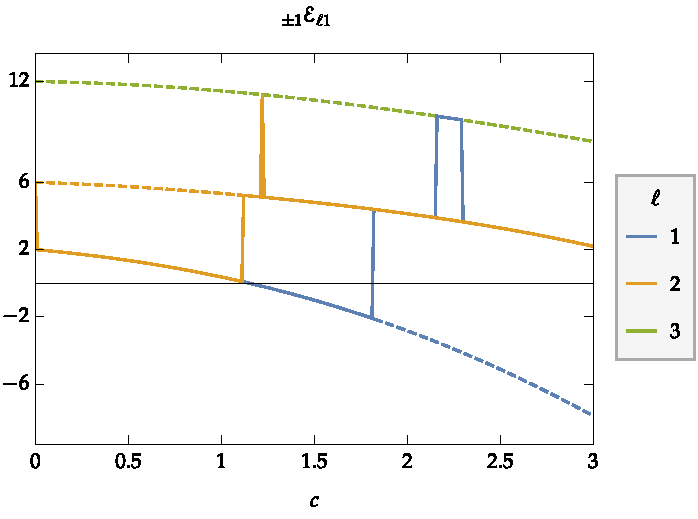
\includegraphics[width=\textwidth]{discontinuitiesEV}
    \end{subfigure}
	\caption{Showcasing discontinuities in the values of $\uu[\pm 1]{\mathscr{E}}{\ell 1}$ for $m=1,2$ when using an incorrect implementation of the Leaver method. Real values of the eigenvalues are shown as dashed lines ($m=1,2,3$) of the same color.}
	\label{fig4:discontinuitiesEV}
\end{figure}
For a fixed $s$ and $m$, we have an infinite number of curves labeled by $\ell$ and in some cases the root finding algorithm selects roots from adjacent curves, either from the branch $\ell-1$, $\ell+1$ or even distant values.
These solutions cannot ever intersect, otherwise the eigenvalue would be degenerate and the SWSHs would not be a orthogonal basis of functions.
The issue rests on the lack of accuracy when identifying of the $\ell$-th root.
We lose accuracy when trying to obtain roots on levels further down in the continued fraction.
We solve the problem by considering the inversion \eref{eq3:evInversionRth}, choosing $r=\ell+\max\{|m|,|s|\}$, as the main information in the value taken by the $\ell$-th root is in the $\beta_r$ coefficient, with the continuous fractions providing higher order contributions in $c$.

Once the eigenvalue root is known, one can find any number of the series expansions coefficients $a_p$, for a particular eigenfunction \eref{eq3:SWSHseriesLeaver}, by using the three-coefficient recursion relation \eref{eq3:ap3CoefRecursion}.

%-----------------------------------------------------------------------------------

\subsection{Spectral method}

Due to initial problems with the Leaver method, we decided to use the spectral method \cite{Cook2014},
since the spheroidal \eqref{eq3:teukolskyAngular} can be seen as a perturbed version of the spherical case, $c=0$.
We may rewrite the equation using three operators depending on their order in $c$, 
\begin{align}
	\label{eq4:angularEqH012}
	( \mathscr{H}^{(0)} +  \mathscr{H}^{(1)} + \mathscr{H}^{(2)} ) \uu[s]{S}{\ell m} = - \uu[s]{\mathscr{E}}{\ell m}  \;\uu[s]{S}{\ell m} 
\end{align}
The zeroth order operator, $\mathscr{H}^{(0)}$, defines the eigenvalue problem for the spin-weighted spherical harmonics, which will provide the complete non-perturbed basis, $\mathscr{H}^{(0)} \,\uu[s]{Y}{\ell m} = -\ell(\ell+1) \,\uu[s]{Y}{\ell m}$.
The other two operators are quickly identified from the angular equation as $\mathscr{H}^{(1)} = - 2 s c \cos\theta$ and $\mathscr{H}^{(2)} = c^2 \cos^2\theta$.
Simple perturbation theory \cite{TeukolskyPress1973b} states that
\begin{align}
	\begin{split}
		\uu[s]{\mathscr{E}}{\ell m} &= \ell(\ell+1) - \int \dd\Omega \,(\uu[s]{Y}{\ell m})^* \,\mathscr{H}^{(1)} \,\uu[s]{Y}{\ell m} + \mathscr{O}(c^2) ~, \\
		\uu[s]{S}{\ell m} &= \uu[s]{Y}{\ell m} - \sum_{j\ne\ell} \frac{\int \dd\Omega \,(\uu[s]{Y}{j m})^* \,\mathscr{H}^{(1)} \,\uu[s]{Y}{\ell m}}{j(j+1)-\ell(\ell+1)} \, \uu[s]{Y}{j m} +\mathscr{O}(c^2) ~.
	\end{split}
\end{align}
We may include $\mathscr{H}^{(2)}$ by using a higher order expansion, which can be found in any Quantum Mechanics textbook.
The integrals $\int \dd\Omega \,(\uu[s]{Y}{j m})^* \,\mathscr{H}^{(1)} \,\uu[s]{Y}{\ell m}$ and $\int \dd\Omega \,(\uu[s]{Y}{j m})^* \,\mathscr{H}^{(2)} \,\uu[s]{Y}{\ell m}$ may be computed using Clebsch-Gordon coefficients decomposition generalized for spin-weighted harmonics \eref{eqC:clebschGordanDecomp}.
These operators can be written in terms of general matrix elements in the basis of spin-weighted spherical harmonics \cite{TorresdelCastillo2003},
\begin{align}
	\begin{split}
	h^{(1)}_{j\ell} &= \int \dd\Omega \,\cos\theta \,(\uu[s]{Y}{j m})^* \,\uu[s]{Y}{\ell m} = \sqrt{\frac{2 \ell+1}{2 j+1}} \langle \ell,m; 1,0 | j,m \rangle \langle \ell, -s; 1,0 | j, -s \rangle ~, \\
	h^{(2)}_{j\ell} &= \int \dd\Omega \,\cos^2\theta \,(\uu[s]{Y}{j m})^* \,\uu[s]{Y}{\ell m} = \frac{\delta_{j\ell}}{3} + \frac{2}{3}\sqrt{\frac{2 \ell+1}{2 j+1}} \langle \ell,m; 2,0 | j,m \rangle \langle \ell, -s; 2,0 | j, -s \rangle ~,
	\end{split}
\end{align}
remembering that $\cos\theta$ and $\cos^2\theta$ can be rewritten using $\uu[0]{Y}{10}(\theta,\varphi)$ and $\uu[0]{Y}{20}(\theta,\varphi)$.
The first integral is proportional to the Leaver series coefficient $f_1$ defined in~\aref{AppendixEigenvalues}.

Perturbation theory shows that the SWSHs can be expanded in terms of spherical harmonics.
This should not be a surprising fact as any angular function $f(\theta,\varphi)$ with a particular spin-weight can be represented using a decomposition using spin-weighted spherical harmonics.
Having this idea in mind, we write 
\begin{align}
	\label{eq4:SWSHsphericalExpansion}
	\uu[s]{S}{\ell m}(c; \theta, \varphi) = \sum_{j} b_{j}^{(\ell)} \,\uu[s]{Y}{j m}(\theta,\varphi) \qquad \Big( \ell, j \ge \max\{|s|,|m|\} \Big) ~.
\end{align}
Replacing the expansion in \eqref{eq4:angularEqH012}, we can take advantage of the orthogonality of the harmonics, $\int \dd\Omega \,(\uu[s]{Y}{j m})^* \,\uu[s]{Y}{\ell m} = \delta_{\ell j}$, by multiplying the the equation by $(\uu[s]{Y}{\ell m})^*$ and integrating the solid angle.
The angular equation is replaced by an eigenvalue matrix equation $\sum_{j} a_{ij} \, b_{j}^{(\ell)} = - \uu[s]{\mathscr{E}}{\ell m} \,b_{i}^{(\ell)}$, such that
\begin{equation}
	\label{eq4:spectralMatrix}
	a_{ij} =
	\begin{cases} 
		~c^2 \,h^{(2)}_{ii} - 2 s c \,h^{(1)}_{ii} - i(i+1) & ~ i=j \\[-0.5ex]
		~c^2 \,h^{(2)}_{ij} - 2 s c \,h^{(1)}_{ij} & ~ |i-j|=1 \\[-0.5ex]
		~c^2 \,h^{(2)}_{ij} & ~ |i-j|=2 \\[-0.5ex]
		~0 & ~\text{otherwise}
	\end{cases}  \qquad \Big( i, j \ge \max\{|s|,|m|\} \Big) ~,
\end{equation}
where the the eigenvalues of this matrix are $-\uu[s]{\mathscr{E}}{\ell m}$ and the correspondent eigenvector is given by $b_j^{(\ell)}$.

Like the Leaver method, we will have to truncate the matrix at some finite size.
From \eqref{eq4:spectralMatrix}, we know that the zeroth order contribution to the $\ell$-th eigenvalue will be the element $a_{\ell\ell}$.
We opted to implement a $N\times N$ centered submatrix such that $i,j\ge\ell_\mathrm{\min}\equiv\max\{|s|,|m|\}$ and truncating the matrix at $N > \ell+1 - \ell_\mathrm{\min}$, in order to include the $a_{\ell\ell}$ terms in the approximation.
In reality, we must implement a variable $N\equiv N(c)$, so that it increases the size of the taken submatrix in order to include extra corrections for larger values of $c$.
The size of the submatrix also increases linearly with $\ell$.
The best way to approximate $\uu[s]{\mathscr{E}}{\ell m}$ would be to not construct the submatrix including all values of $\ell_\mathrm{\min}$ but instead to center the submatrix at $a_{\ell\ell}$ and increase its size to fine-tune the eigenvalue.
Since we will take very large $\ell$ values, we will use the first method for simplicity.

\begin{figure}[h]
	\centering
	\vspace{0.2cm}
	\begin{subfigure}[c]{0.49\textwidth}
        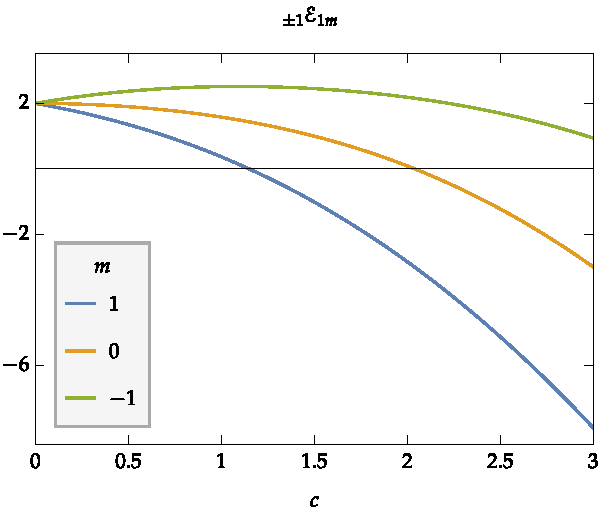
\includegraphics[width=\textwidth]{plotEV1}
	\end{subfigure}
	\hfill
	\begin{subfigure}[c]{0.48\textwidth}
		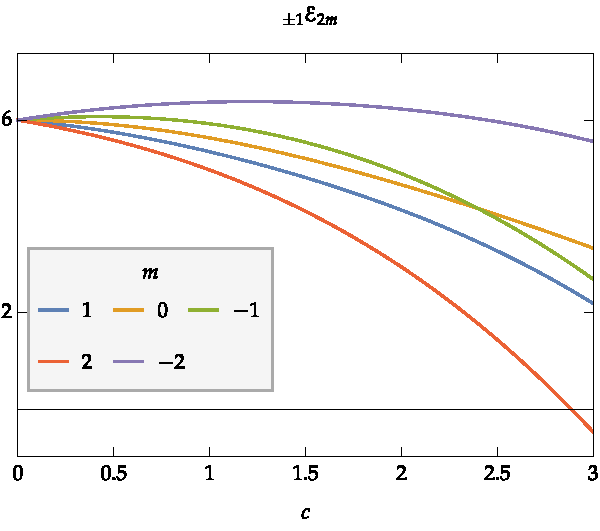
\includegraphics[width=\textwidth]{plotEV2}
	\end{subfigure}
	\hfill
	\caption{Eigenvalues for $\ell=1$ (left) and $\ell=2$ (right) for typical values of $c$, using the spectral method.}
	\label{fig4:plotsEV12}
\end{figure}
Optimized numerical methods allow for fast computation of the eigenvalues and eigenvectors of a band-diagonal matrix.
The ``Eigensystem'' method found in Mathematica\texttrademark~ returns an array of eigenvalues and their correspondent normalized eigenvectors, guaranteeing \eqref{eq3:SWSHorthogonality}. Since the result is a positively sorted list of $-\uu[s]{\mathscr{E}}{\ell m}$, with $0\le \ell-\ell_\mathrm{min}\le N-1$, of which we need to select the negative of the ($N-\ell+\ell_\mathrm{min}$)-th element.
We show EM eigenvalues form lower $\ell$ values in \fref{fig4:plotsEV12}.
\begin{figure}[!b]
	\centering
	\vspace{0.2cm}
	\begin{subfigure}[c]{0.49\textwidth}
        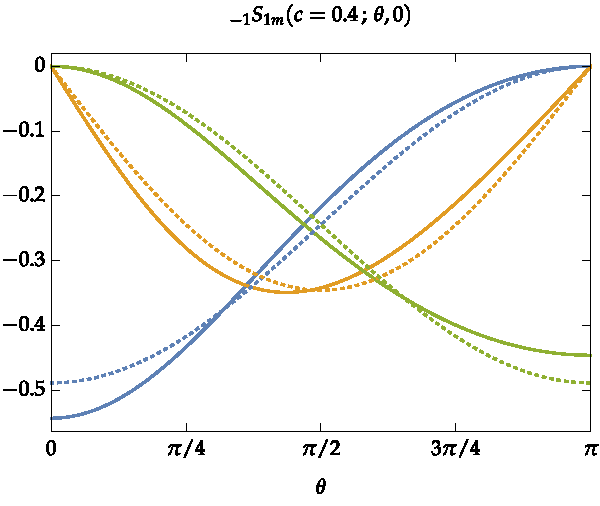
\includegraphics[width=\textwidth]{plotSWSH1}
	\end{subfigure}
	\hfill
	\begin{subfigure}[c]{0.49\textwidth}
		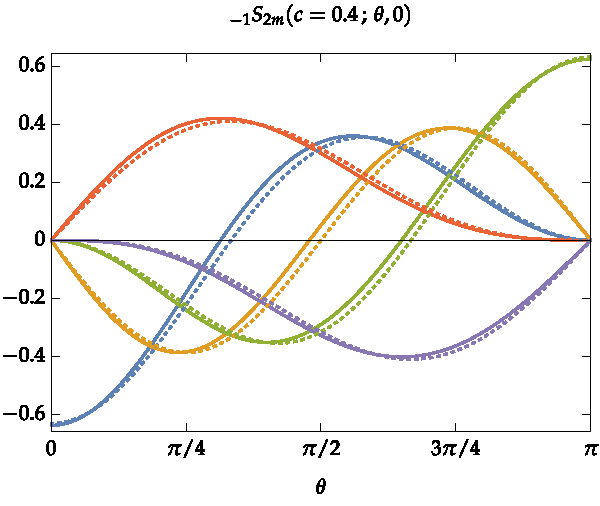
\includegraphics[width=\textwidth]{plotSWSH2}
	\end{subfigure}
	\hfill
	\caption{Plots of all spin-weighted spheroidal harmonics $\uu[-1]{S}{\ell m}(\theta,0)$ with $\ell=1$ (left) and $\ell=2$ (right) for $s=-1$ and $c=0.4$. This plot shares the same legend coloring as the above (\fref{fig4:plotsEV12}). Dotted curves represent the values of the $\uu[-1]{Y}{\ell m}$, when $c\to0$.}
	\label{fig4:plotSWSH12}
\end{figure}
This procedure also returns correct eigenvectors for approximating the eigenfunction using \eref{eq4:SWSHsphericalExpansion}.
In order to ensure that the SWSHs have the same phase convections of their spherical counterparts, we must ensure that the correspondent eigenvector has $b_\ell^{(\ell)}>0$, by mapping the obtained vector components as $b_j^{(\ell)}\mapsto \mathrm{sgn}(b_\ell^{(\ell)}) \,b_j^{(\ell)}$.
This process is computationally more stressful, since it requires computing and combining $N$ different spherical harmonics with the same $s$ and $m$.
In the superradiance range, the values of $c$ can be small $\left(<\tfrac{1}{2}|m|\right)$, therefore the SWSHs may not differ greatly from $\uu[s]{Y}{\ell m}(\theta,\varphi)$, with smaller deviations as $\ell$ increases (e.g. see \fref{fig4:plotSWSH12}).
In this regime, we may the use pure spin-weighted spherical harmonics as approximations, as they do not change the qualitative behaviour of the $\uu[s]{S}{\ell m}(\theta,\varphi)$.

%-----------------------------------------------------------------------------------

\section{Amplification factor}

Finding non-approximate forms to the amplification factor $\uu[\pm 1]{Z}{\ell m}$ requires the numerical solving of the radial \eqref{eq3:radialTeukolskyAdimensional}, which is already in an adimensional form.
We computed the angular eigenvalues beforehand, which depend on the mode $(\ell,m)$ as well as the coupling $c=a\omega$.
Additionally the equation depends on the BH parameters $(M,J)$ and $\omega$ explicitly, but it is possible to normalize all variables so that we only need to specify $(\mathscr{J}, \ell, m, \bar{\omega})$, where $\mathscr{J}=a/M=J/M^2$.
We choose to work with barred frequencies because $\bar{\Omega}_H = \mathscr{J}/2$, which makes it easier to numerically select superradiant modes.

We need to obtain numerical interpolations for $\uu[\pm 1]{R}{\ell m}$, by integrating the solution outwards from the horizon, at $x=0$, up to a sufficiently large $x_\infty \gg |\bar{\omega}|^{-1}$. 
The solutions for $s=\pm 1$ contain the all the EM field information, but they have different asymptotic behaviors.
For $\phi_0$, \eqref{eq3:asymptoticR} tells us that the ingoing coefficient tends to overshadow the outgoing coefficient, while the opposite occurs for $\phi_2$.
This way seems natural to try to solve both equations, where we can obtain $\mathscr{Y}_\mathrm{in}$ and $\mathscr{Z}_\mathrm{out}$ separately (\tref{tb3:approximatedRsolutionsYZ}).

Knowing the irregularities of the solution at the horizon, we propose the ansatz
\begin{align}
	\label{eq4:numericalRansatz}
	\uu[\pm 1]{R}{\ell m} = (r_+)^{\mp 1} \, x^{ \mp 1 - i \varpi / \tau} f_{\pm}(x) ~,
\end{align}
where $f(x)$ is a new function that obeys a regular second-order differential equation.
Thus we need to set two initial conditions at the horizon, $f_{\pm}(0)$ and $f_{\pm}{\!}'(0)$.
We expect to $|f_\pm(x)|$ to become approximately constant at large $x$, because this
form is written in way a that also matches the behavior of the radial function at infinity, $\uu[\pm 1]{R}{\ell m}\sim r^{\mp 1}$.

Comparing \eqref{eq4:numericalRansatz} with the asymptotic form at large $x$ as well as near the horizon form, we obtain
\begin{align}
	\label{eq4:YinZoutFInf}
	\begin{split}
		r_{+} \tau \,\frac{\mathscr{Y}_\mathrm{in}}{\mathscr{Y}_\mathrm{hole}} &= \frac{f_{+}(x_\infty)}{f_{+}(0)} \exp\left[ - i \bar{\omega} x_\infty - i \bar{\omega} (2-\tau)\log(x_\infty)   -i \frac{\varpi}{\tau} \log(x_\infty) \right] ~, \\[0.15cm]
		\frac{1}{r_{+} \tau} \,\frac{\mathscr{Z}_\mathrm{out}}{\mathscr{Z}_\mathrm{hole}} &= \frac{f_{-}(x_\infty)}{f_{-}(0)} \exp\left[ + i \bar{\omega} x_\infty + i \bar{\omega} (2-\tau)\log(x_\infty) -i \frac{\varpi}{\tau} \log(x_\infty) \right] ~.
	\end{split}
\end{align}
If both solutions are normalized such that $f_{\pm}(0) = 1$, then we have to deal with the relative normalization of $\mathscr{Z}_\mathrm{hole}/\mathscr{Y}_\mathrm{hole}$ \cite{Teukolsky1974}. We can obtain such ratio in terms of known parameters by considering \eqref{eq3:separationB} at $x\simeq0$,
\begin{align}
	(r_{+} \tau)^2 \,\frac{\mathscr{Z}_\mathrm{hole}}{\mathscr{Y}_\mathrm{hole}} = -\frac{\mathscr{B} \tau^2 }{2 \varpi (i \tau + 2 \varpi)} ~.
\end{align}
Therefore to compute the amplification factor we use ($f_{\pm}(0)=1$)
\begin{align}
	\label{eq4:ZFPlusMinus}
	\uu[\pm 1]{Z}{\ell m} = \frac{\mathscr{B}^2 \tau^4 }{4 \varpi^2 (\tau^2 + 4 \varpi^2)} \left| \frac{f_{-}(x_\infty)}{f_{+}(x_\infty)} \right|^2 - 1 ~.
\end{align}

Another way of dealing with the relative normalization would be to select different initial conditions at the horizon $x=0$.
We could cancel the relative normalization of $\mathscr{Z}_\mathrm{hole}/\mathscr{Y}_\mathrm{hole}$ if we set any normalization that results in $f_{-}(0)/f_{+}(0) = -\mathscr{B} \tau^2 /[2 \varpi (i \tau + 2 \varpi)]$, eliminating the dependence on $\mathscr{B}$, $\tau$, $\varpi$ in \eqref{eq4:ZFPlusMinus}.

The differential equation obtained from substituting \eref{eq4:numericalRansatz} into \eqref{eq3:radialTeukolskyAdimensional} is identically zero for $x=0$.
Therefore, no matter what initial conditions set for $f_{\pm}{\!}'$, the system would not evolve due to stiffness, which makes the step size of the integrator effectively zero.
The usual solution for stiff differential equations is to start the solver at a small distance from the horizon $\epsilon>0$.
We adjust the initial conditions by substituting the series expansion of $f_{\pm}(x) = \sum_{n=0}^{N_H} a_n x^n$ in the radial equation, discarding terms higher than $\mathscr{O}(x^{N_H})$ and obtaining the coefficients $a_n \propto a_0$, $1 \le n \le N_H$, like is done in \cite{Rosa2017}. 
Therefore we may set the initial conditions as
\begin{align}
	f_{\pm}(\epsilon) = f_{\pm}(0) \sum_{n=0}^{N_H} \left(\frac{a_n}{a_0}\right) \epsilon^n ~,\qquad f_{\pm}{\!}'(\epsilon) = f_{\pm}(0) \sum_{n=1}^{N_H} \left(\frac{a_n}{a_0}\right) \epsilon^n ~,
\end{align}
where $f_{\pm}(0)=1$ are the original horizon conditions considered.
We found $\epsilon=10^{-12}$, $N_H=6$ and $x_\infty = 200 \times 2\pi/|\bar{\omega}|$ working perfectly for the ``NDSolve'' integrator.
Effectively we will have $|f_{\pm}{\!}'(\epsilon)|\simeq \epsilon$, but this contribution is sufficient to remove stiffness from the system and has important contributions in the case of extremal BHs ($\mathscr{J}\to 1$).

This previous method requires us to call the integrator twice which is not very effective numerically.
Exploring the conservation of the Wronskian (conserved current) of \eqref{eq3:D2PlusVeff}, we can obtain \cite{Teukolsky1974}
\begin{align}
	\label{eq4:InOutHole}
	\frac{\dd E_\mathrm{in}}{\dd t} - \frac{\dd E_\mathrm{out}}{\dd t} = \frac{\dd E_\mathrm{hole}}{\dd t} ~,
\end{align}
which simply states total energy conservation.
Therefore we can rewrite \eqref{eq3:Zdef} using only the \emph{hole-in} ratio, thus we are able to get the amplification factor with just with the $s=+1$ solution,
\begin{align}
	\label{eq4:ZFPlusPlus}
	\uu[\pm 1]{Z}{\ell m} = - \frac{\bar{\omega} \tau^2}{\varpi} \left|\frac{f_{+}(0)}{f_{+}(x_\infty)}\right|^2 ~.
\end{align}
If we use the \emph{out-hole} ratio in the amplification factor we only need to solve for $s=-1$,
\begin{align}
	\label{eq4:ZFMinusMinus}
	\uu[\pm 1]{Z}{\ell m} = - \left( 1 + \frac{\mathscr{B}^2 \tau^2}{4 \bar{\omega} \varpi(\tau^2 + 4 \varpi^2)} \left|\frac{f_{-}(x_\infty)}{f_{-}(0)}\right|^2 \right)^{-1} ~.
\end{align}
For the mode $\ell=m=1$ at $\mathscr{J}=0.9999$, we obtain the maximum amplification of about $4.36\%$ for a frequency of about $\omega M \simeq 0.436$.
Modes in the region \eref{eq3:superradiance} have always $\uu[\pm 1]{Z}{\ell m}>0$, but the amplification factor decreases quickly as $\ell$ increases (\fref{fig4:logZ}).~
For frequencies where $|\omega|>|m\Omega_H|$, we obtain that the value of $\uu[\pm 1]{Z}{\ell m} \to -1$.
\begin{figure}[h]
	\centering
	\vspace{0.2cm}
	\begin{subfigure}[c]{0.6\textwidth}
        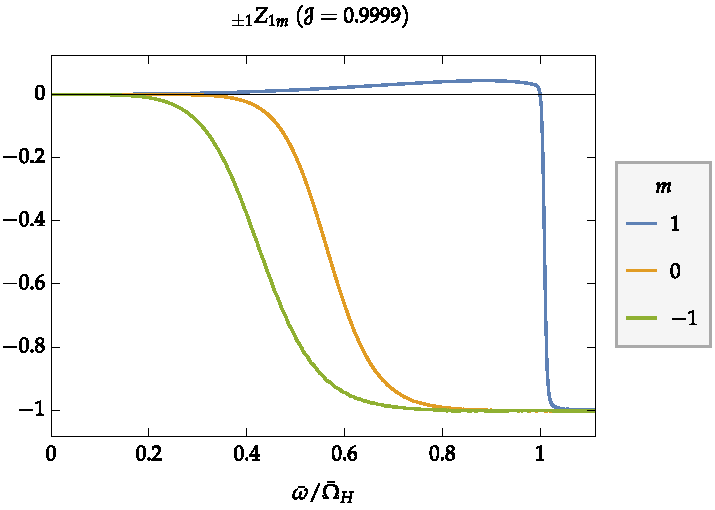
\includegraphics[width=\textwidth]{precisionZ1}
	\end{subfigure}
	\caption{Amplification factor of an extremal BH ($\mathscr{J}=0.9999$) for modes with $\ell=1$. In this figure, superradiance occurs only for $m=1$ as predicted.}
	\label{fig4:plotZ11}
\end{figure}
This in no surprising fact because as $\omega$ increases so does the ingoing wave energy. Therefore when crossing the superradiant threshold the wave possesses enough energy to cross the $V_\mathrm{eff}$ barrier, being absorbed by the BH.

Thus we have three ways of computing $\uu[\pm 1]{Z}{\ell m}$, but only two of them are independent.
We rename these different forms in Eqs. \eref{eq4:ZFPlusPlus}, \eref{eq4:ZFMinusMinus}, \eref{eq4:ZFPlusMinus} as $Z^{(1)}$, $Z^{(2)}$, $Z^{(3)}$, respectively.
We can rearrange the RHS of the expressions so that we have
\begin{align}
	Z^{(3)} = Z^{(1)} \left[ 1 + \frac{1}{Z^{(2)}} \right] - 1 ~.
\end{align}
It is expected that if the amplification factors based only on a single solution for $\phi_0$ or $\phi_2$ are approximately equal, then the same would be true when considering $Z^{(3)}$, which uses both solutions.
However, from a closer look at \fref{fig4:plotZ53} we can see that this is not true, especially for higher values of $\ell$.
\begin{figure}[h]
	\centering
	\vspace{0.2cm}
	\begin{subfigure}[c]{0.6\textwidth}
        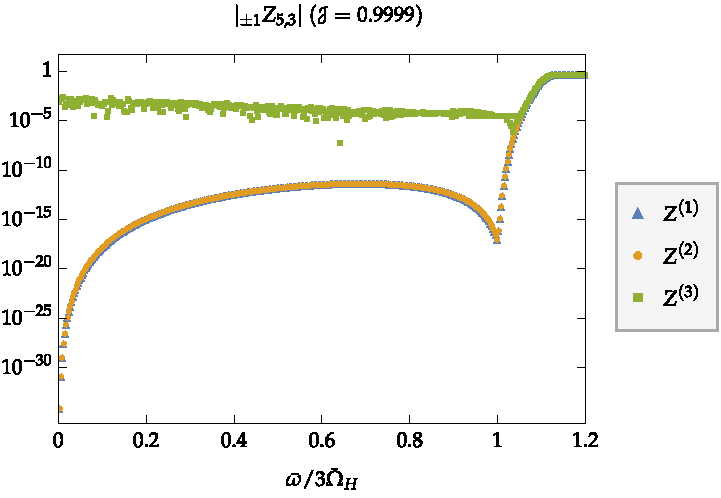
\includegraphics[width=\textwidth]{noPrecisionZ53}
	\end{subfigure}
	\caption{Log plot demonstrating error propagation for $\uu[\pm 1]{Z}{53}$ when computing the factor using both numerical solutions for the radial part of $\phi_0$ and $\phi_2$.}
	\label{fig4:plotZ53}
\end{figure}
Somehow it appears that we are not able to compute the ratio of $\mathscr{Y}_\mathrm{in}$ and $\mathscr{Z}_\mathrm{out}$ with enough accuracy, probably because the large values that $f_{\pm}(x_\infty)$ take do not hold the necessary precision to compute their ratio accurately.

To better understand this, let us choose a superradiant frequency. For larger values of $\ell$ (with small $m$) the gain/loss factor is practically zero.
Still we have huge differences in the order of magnitude of the amplification factor when comparing results from using only one solution and using both.
Since two different equations are numerically solved, there will always be a discrepancy due to the independent numerical solutions, $Z^{(2)} = Z^{(1)} (1+\eta)$, with $\eta$ very small.
The problem is that this error is propagated in absolute value, $Z^{(3)} \simeq Z^{(1)} - \eta$.
For example, when $(\mathscr{J}, \ell, m, \bar{\omega})=(0.9999,5,3,0.1)$ we have $\eta \simeq -0.003$ and $Z^{(1)}\sim 10^{-20}$, which implies that when using both solutions we have a discrepancy of a factor of $10^{17}$.
Therefore we cannot use the expression $Z^{(3)}$ to accurately compute the amplification factor, when we have $\eta \gg Z^{(1)} , Z^{(2)}$.

We further to increase the numerical precision in this problem by considering higher order terms in the asymptotic expansion of \eqref{eq3:asymptoticR}.
Separately, we will substitute both asymptotic series in \eqref{eq3:radialTeukolskyAdimensional}, one for the ingoing part and another for the outgoing \cite{Brito2015}.
Together they have the form
\begin{align}
	\label{eq4:radialIOseries}
	\uu[-1]{R}{\ell m}(r) &= e^{-i \bar{\omega} x}  \, x^{ - 1 - i (2-\tau) \bar{\omega} } \sum_{n=0}^{N_\infty} I_n \, x^{-n} + \, e^{-i \bar{\omega} x} x^{ 1 + i (2-\tau) \bar{\omega} } \sum_{n=0}^{N_\infty} O_n \, x^{-n} ~,
\end{align}
where we identify $I_0 \,r_{+} = \mathscr{Z}_\mathrm{in}/ \mathscr{Z}_\mathrm{hole}$ and $O_0/r_{+} = \mathscr{Z}_\mathrm{out}/\mathscr{Z}_\mathrm{hole}$.
Although we have chosen the $s=-1$ solution, the same procedure can be done for $s=+1$, because when using a higher order expansion, both ingoing and outgoing coefficients are present.

Firstly, we directly substitute the series into \eqref{eq3:radialTeukolskyAdimensional}, neglecting terms above $\mathscr{O}(x^{-N_\infty})$ and grouping the exponentials terms, in order to obtain $I_n\propto I_0$, $O_n\propto O_0$ ($1 \le n \le N_\infty$), exactly like the series used above to define boundary conditions at the horizon.
Secondly, substitution of the numerical ansatz \eref{eq4:numericalRansatz} in the LHS of the previous equation, together with its derivative, we have a system of two linear equations, which in the limit of large-$x$ limit allows to determine
\begin{align}
	\frac{1}{r_+} \,\frac{\mathscr{Z}_\mathrm{in}}{\mathscr{Z}_\mathrm{hole}} = I_0\Big( f_{-}(x_\infty), \,f_{-}{\!}'(x_\infty) \Big) ~,\qquad r_{+} \frac{\mathscr{Z}_\mathrm{out}}{\mathscr{Z}_\mathrm{hole}} = O_0\Big( f_{-}(x_\infty), \, f_{-}{\!}'(x_\infty) \Big) ~.
\end{align}
Lastly, we may use the previous expression \eref{eq4:InOutHole} to compute $\uu[\pm1]{Z}{\ell m}$ using only one of the coefficient, instead of using \eqref{eq3:amplificationBAoutAin}. 
This new method solves some of the precision problems from the initial implementation when using both $\phi_0$ and $\phi_2$, for a smaller $x_\infty = 80 \times 2 \pi / |\bar{\omega}|$ and $N_\infty = 10$, with the same $\epsilon = 10^{-12}$.

A similar method is implemented in \cite{Brito2015}, which is very similar with the obtained results.
These are very similar to those of Teukolsky \cite{TeukolskyPress1973b}.
By identifying the source of the problem as the error propagation in expression \eref{eq4:ZFPlusMinus}, we are now aware that we must use definitions of $\uu[\pm 1]{Z}{\ell m}$ that have either \emph{in} or \emph{out} coefficient.
Therefore we are able to obtain result with more precision and less noise compared to data originated from other methods (e.g. compare with \cite{Brito2015}).

In \fref{fig4:logZ}, we have the logarithm-scaled plot of the amplification factor for different superradiant modes. We can infer that $\uu[\pm 1]{Z}{\ell m}$ decreases in order of magnitude as $\ell$ increases.
Therefore the mode with the highest amplification factor is $\ell=m=1$, we is plotted in detail in \fref{fig4:plotZ11}.
This particular plot reveals information which most relevent when considering a wave which is a superposition of harmonic modes.
\begin{figure}[t]
	\centering
	\begin{subfigure}[c]{0.9\textwidth}
        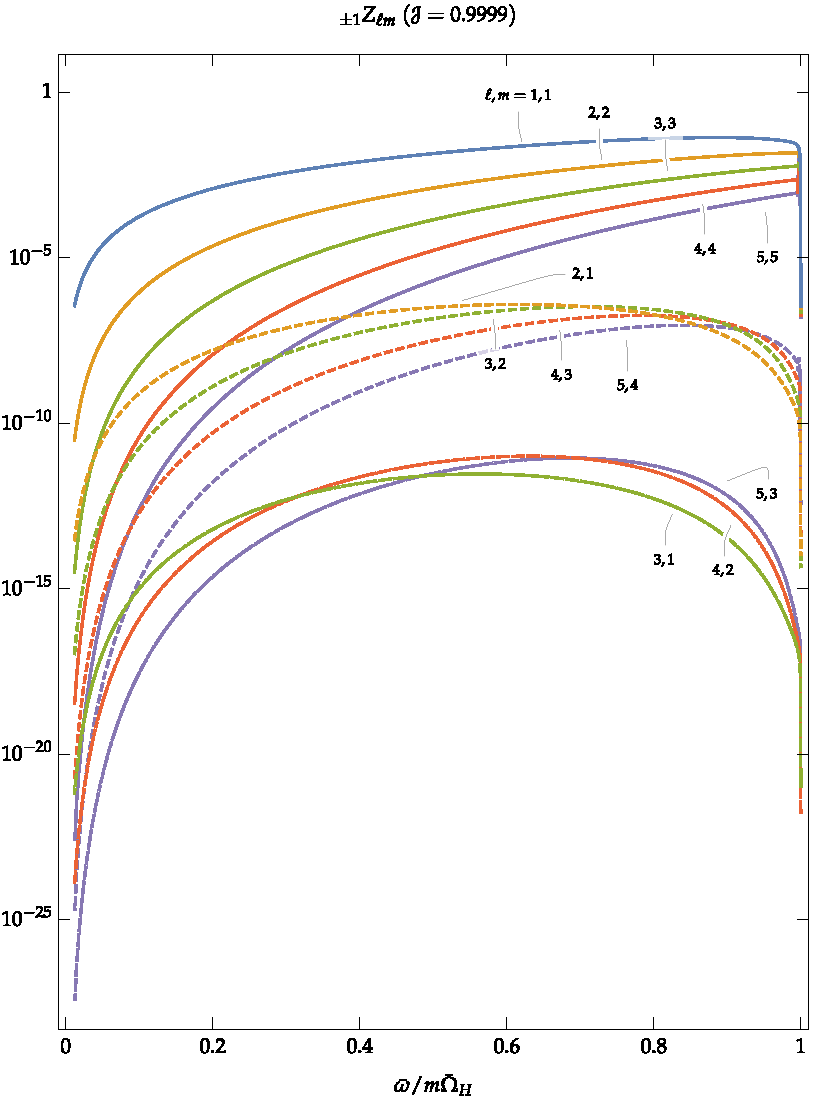
\includegraphics[width=\textwidth]{precisionLogZ}
	\end{subfigure}
	\caption{Log plot of $\uu[\pm 1]{Z}{\ell m}$ as a function of $\bar{\omega}/m\bar{\omega}_H$ \cite{TeukolskyPress1973b}. Each color represents the same value of $\ell$, while different dashing corresponds to grouping the modes as $|\ell-m|=0,1,2$.}
	\label{fig4:logZ}
\end{figure}

%-----------------------------------------------------------------------------------

\cleardoublepage